%% ===========================================================================
%%  GB-META -- manuscript source.
%%  IEEE conference format (IEEEtran). Target: 6 pages.
%%
%%  Build:
%%      pdflatex GB_META_v2 && bibtex GB_META_v2 && pdflatex GB_META_v2 x2
%%
%%  Every table is \input from paper/tex/, generated by
%%  scripts/make_paper_tex.py directly from the result CSVs. Do not edit
%%  numbers here -- regenerate them, so the manuscript cannot drift from the
%%  artefacts it reports.
%% ===========================================================================
\documentclass[conference]{IEEEtran}
\IEEEoverridecommandlockouts

\usepackage{cite}
\usepackage{amsmath,amssymb}
\usepackage{graphicx}
\usepackage{booktabs}
\usepackage{url}
\usepackage[hidelinks]{hyperref}

\graphicspath{{figures/}}

% This paper is float-heavy (six tables, two figures, three of them spanning
% both columns). With LaTeX's defaults, two-column floats are deferred and pile
% up, padding the body with whitespace. Allowing denser float packing, and
% trimming the generous default separation around each float, is what keeps the
% paper at six pages.
\setlength{\textfloatsep}{8pt plus 2pt minus 2pt}
\setlength{\floatsep}{8pt plus 2pt minus 2pt}
\setlength{\intextsep}{8pt plus 2pt minus 2pt}
\setlength{\dblfloatsep}{8pt plus 2pt minus 2pt}
\setlength{\dbltextfloatsep}{8pt plus 2pt minus 2pt}
\renewcommand{\topfraction}{0.92}
\renewcommand{\bottomfraction}{0.85}
\renewcommand{\textfraction}{0.06}
\renewcommand{\floatpagefraction}{0.80}
\renewcommand{\dbltopfraction}{0.92}
\renewcommand{\dblfloatpagefraction}{0.80}
\setcounter{topnumber}{3}
\setcounter{bottomnumber}{2}
\setcounter{totalnumber}{5}
\setcounter{dbltopnumber}{3}

\begin{document}

\title{GB-\textsc{Meta}: Gradient-Boosting Meta-Ensemble for IoT/IIoT Intrusion
Detection on Edge-IIoTset}

\author{\IEEEauthorblockN{Jalaj Sharma}
\IEEEauthorblockA{\textit{Centre for Internet of Things} \\
\textit{MITS DU}, Gwalior, India \\
jalajsharma3107@gmail.com}
\and
\IEEEauthorblockN{Ayan Ahmed Khan}
\IEEEauthorblockA{\textit{Centre for Internet of Things} \\
\textit{MITS DU}, Gwalior, India \\
ayan.ahmedkhan591@gmail.com}
\and
\IEEEauthorblockN{Kaushal Pratap Sengar}
\IEEEauthorblockA{\textit{Centre for Internet of Things} \\
\textit{MITS DU}, Gwalior, India \\
kaushalsengar786@gmail.com}}

\maketitle

% ---------------------------------------------------------------------------
\begin{abstract}
This paper presents GB-\textsc{Meta}, a stacked meta-ensemble that combines
LightGBM, XGBoost and CatBoost through a logistic-regression meta-learner fitted
on out-of-fold log-odds, and establishes the conditions under which it holds
using a leakage-audited protocol over four intrusion-detection benchmarks
(Edge-IIoTset, NSL-KDD, ToN-IoT, UNSW-NB15), three seeds, bootstrap intervals and
McNemar, Friedman--Nemenyi and Nadeau--Bengio testing. On Edge-IIoTset
GB-\textsc{Meta} attains the best macro-F1 of eleven models ($0.9225 \pm 0.0026$
over three seeds) and the best calibration of any model tested (ECE 0.0051), with
the margin concentrated in the minority classes; an ablation attributes this to
the learned combination step, since an unweighted soft vote over the same three
learners is 0.0077 macro-F1 worse with an interval excluding zero. The advantage
is benchmark-specific, and we report its limits: a corrected paired $t$-test
across seeds does not separate GB-\textsc{Meta} from its strongest single
component ($+0.0062$, $p{=}0.124$), and on UNSW-NB15 a single LightGBM is
significantly better ($-0.0214$, $p{=}0.005$). The audit behind this scope finds
exact-duplicate rates from 0.0\% to 38.6\% across the four benchmarks, and a
perturbation analysis finds CatBoost alone more stable than the ensemble built on
it. We recommend GB-\textsc{Meta} where calibrated minority-class detection on
IoT traffic is the objective, and release the protocol behind these claims.
\end{abstract}

\begin{IEEEkeywords}
Data leakage, ensemble learning, gradient boosting, imbalanced classification,
intrusion detection, statistical significance
\end{IEEEkeywords}

% ---------------------------------------------------------------------------
\section{Introduction}

IoT deployments in safety-critical settings continue to grow faster than the
security mechanisms built into them, and signature-based intrusion detection
generalises poorly to the attack patterns these networks
exhibit~\cite{ferrag2022edgeiiotset}. Gradient-boosted tree models have
consequently become the dominant approach for tabular network-flow detection, and
stacked ensembles of them are routinely reported above 99\% accuracy on
Edge-IIoTset.

Those figures are, however, almost never accompanied by a confidence interval, a
significance test, or an audit of the data on which they were measured. On the
standard 157{,}800-row Edge-IIoTset split, one tenth of an accuracy point is
about 158 test rows, and the MITM class contains 72 test rows in total, so a
single flipped prediction moves its per-class F1 by roughly 1.4 points. The
differences by which published detectors separate themselves are of that
magnitude.

\subsection{Contributions}

\begin{itemize}
\item \textbf{C1. Leakage-free, audited preprocessing.} All statistics are fitted
on training rows only, duplicates are removed globally before splitting, and
three audit probes (duplicate rate, encoded train/test overlap with its
memorisation ceiling, and single-feature predictability) are reported for every
benchmark (Table~\ref{tab:datasets}).
\item \textbf{C2. GB-\textsc{Meta}}, a logistic-regression stack over three
gradient-boosted learners built on out-of-fold meta-features, evaluated on four
benchmarks (Table~\ref{tab:main}).
\item \textbf{C3. Statistical validation.} McNemar's exact test, paired
percentile bootstrap intervals, Friedman with the Iman--Davenport correction,
Nemenyi post-hoc analysis and the Nadeau--Bengio corrected paired $t$-test, all
Holm-corrected (Table~\ref{tab:headline}, Fig.~\ref{fig:cd}).
\item \textbf{C4. Component ablation} isolating the contribution of each base
learner, of the learned combination step against a soft vote, and of the
meta-feature transform, each with a bootstrap interval
(Table~\ref{tab:ablation}).
\item \textbf{C5. Deployment cost profile}: batch-1 latency percentiles,
throughput, serialised size and training cost, measured end to end for the stack
(Table~\ref{tab:cost}).
\item \textbf{C6. Robustness and drift analysis}: macro-F1 under input
perturbation, which separates the models far more sharply than clean accuracy
does, and a chronological analysis showing that ToN-IoT's temporal split is
class-disjoint and therefore cannot support a drift experiment.
\end{itemize}

% ---------------------------------------------------------------------------
\section{Related Work}

\textbf{Gradient-boosted and stacked IDS.} XGBoost~\cite{chen2016xgboost},
LightGBM~\cite{ke2017lightgbm} and CatBoost~\cite{prokhorenkova2018catboost} are
established for tabular intrusion detection, and stacking~\cite{wolpert1992stacked}
is a standard way to combine them. On Edge-IIoTset, Gaber and
Nechaevskiy~\cite{gaber2025xcl} soft-vote the same three learners and report
100\% accuracy, though binary and on a balanced subsample. Abdulkareem et
al.~\cite{abdulkareem2024sel} publish a lightweight stacking ensemble, and
Asif~\cite{asif2025osen} optimises one with a genetic algorithm. Ishtiaq et
al.~\cite{ishtiaq2025cstafnet} report 99.97\% on the 15-class task. Ismail et
al.~\cite{ismail2025lightweight} compare stacking across three IIoT benchmarks
with deployment monitoring, reporting micro-F1. None of these works reports a
significance test or a confidence interval, so the ordering among them, and the
conditions under which any of them holds, remain unestablished.

\textbf{Benchmark quality and evaluation.} The Edge-IIoTset authors themselves
drop fifteen identifier columns before
modelling~\cite{ferrag2022edgeiiotset}. Al Nuaimi et
al.~\cite{alnuaimi2023comparative} find the binary task essentially solved while
the multi-class task ``requires more careful treatment''. Arp et
al.~\cite{arp2022dosdonts} catalogue sampling bias, spurious correlations and
inappropriate baselines as pervasive in security ML. Our audit instruments three
of them. For the statistics we follow standard prescriptions:
Dietterich~\cite{dietterich1998tests} for McNemar on a single test set,
Demšar~\cite{demsar2006statistical} for Friedman with Nemenyi across datasets,
and Nadeau and Bengio~\cite{nadeau2003inference} for the variance correction that resampled paired $t$-tests require.

% ---------------------------------------------------------------------------
\section{Datasets and Leakage Audit}
\label{sec:data}

% The file names are long unbreakable \texttt tokens; without the explicit
% \allowbreak points TeX cannot find good line breaks here and sets the whole
% paragraph underfull.
The evaluation uses four public benchmarks, each in its smallest usable published
variant so the whole study fits one GPU session: Edge-IIoTset
(\texttt{ML-\allowbreak EdgeIIoT-\allowbreak dataset.csv})~\cite{ferrag2022edgeiiotset},
NSL-KDD (\texttt{KDDTrain+})~\cite{tavallaee2009nslkdd}, ToN-IoT
(\texttt{Train\_\allowbreak Test\_\allowbreak Network})~\cite{moustafa2021toniot}
and UNSW-NB15~\cite{moustafa2015unswnb15}. Edge-IIoTset and ToN-IoT are
IoT/IIoT captures. NSL-KDD and UNSW-NB15 are general network-intrusion
benchmarks, included deliberately so that transfer is tested off the domain the
stack was tuned on rather than only within it. Each is reduced to 80{,}000 rows
by stratified sampling with a per-class floor, so rare attack classes survive,
and split 68/12/20 into training, validation and test partitions.

\begin{table*}[t]
\centering
\caption{Benchmark characteristics and leakage audit. Column definitions are given in Section~\ref{sec:data}.}
\label{tab:datasets}
\resizebox{\textwidth}{!}{%
\begin{tabular}{lrrrrrrrrrrlr}
\toprule
& \multicolumn{5}{c}{Benchmark} & \multicolumn{7}{c}{Leakage audit} \\
\cmidrule(lr){2-6}\cmidrule(lr){7-13}
Dataset & Rows & Used & Cls. & Feat. & Imb. & Dup.\% & Ovl.\% & Coll.\% & Ceiling & Maj. & Strongest single feature & Acc. \\
\midrule
Edge-IIoTset & 157,800 & 80,000 & 15 & 58 & 45 & 3.6 & 18.7 & 18.6 & 0.342 & 0.157 & \texttt{tcp.ack} & 0.305 \\
NSL-KDD & 125,973 & 80,000 & 14 & 81 & 1412 & 0.0 & 2.7 & 1.8 & 0.547 & 0.530 & \texttt{src\_bytes} & 0.867 \\
ToN-IoT & 461,043 & 80,000 & 10 & 84 & 143 & 18.5 & 56.3 & 52.0 & 0.825 & 0.672 & \texttt{dst\_ip\_bytes} & 0.741 \\
UNSW-NB15 & 175,341 & 80,000 & 10 & 60 & 302 & 38.6 & 8.5 & 6.0 & 0.484 & 0.479 & \texttt{sttl} & 0.628 \\
\bottomrule
\end{tabular}}

\end{table*}


Table~\ref{tab:datasets} reports, per benchmark, the largest-to-smallest class
ratio (\emph{Imb.}), the exact-duplicate rate before splitting (\emph{Dup.}), the
share of test rows whose encoded vector also occurs in training (\emph{Ovl.}) and
of training rows sharing a vector with another (\emph{Coll.}), the memorisation
ceiling those imply, the majority-class accuracy (\emph{Maj.}), and the single
strongest feature with the accuracy it reaches alone. Three probes produce these,
all run before any model is trained. \textbf{Exact duplicates} are
removed globally, before splitting; duplicated flows on opposite sides of a split
convert memorisation into apparent generalisation. Removal \emph{lowers} reported
scores, and the rate is reported alongside them: UNSW-NB15's published
partition is 38.6\% duplicates and ToN-IoT 18.5\%, while NSL-KDD, explicitly
constructed by de-duplicating KDD'99, contains none, which independently
confirms the probe. \textbf{Single-feature predictability} fits a depth-3 decision
tree on each feature alone: on NSL-KDD, \texttt{src\_bytes} by itself reaches
86.7\% against a 53.0\% majority baseline.

\textbf{Label-bearing columns} are removed from all four benchmarks, not only the
one where they are best known. Three of the four ship a binary attack indicator
alongside the multi-class label (\texttt{Attack\_label} on Edge-IIoTset,
\texttt{label} on ToN-IoT and UNSW-NB15). Retaining it reduces the multi-class
task to naming the attack given that one is present, and each is dropped by the
dataset specification before any model sees the matrix. NSL-KDD carries no such
indicator but does carry \texttt{difficulty}, the number of 21 reference
classifiers that labelled the row correctly, which is a direct function of the
target and is likewise dropped. ToN-IoT additionally ships free-text fields that
name the attack outright in DNS, TLS and HTTP payload columns, and these are
dropped with the identifiers. The audit is therefore uniform across benchmarks,
which matters because a leakage result reported for one dataset says nothing
about the others.

\textbf{Train/test overlap} measures how many test rows share an encoded feature
vector with a training row. This is not duplicated raw data but a consequence of
dropping the identifier columns, which collapses distinct flows onto identical
vectors. Because a bare overlap rate is easy to over-read, we convert it into the
quantity that bounds the claim: the \emph{ceiling} column of
Table~\ref{tab:datasets}, the accuracy of a classifier answering every overlapped
test row by lookup and every other row with the majority class. Edge-IIoTset's
ceiling is 0.342 against models at 0.945, so memorisation is not the explanation
there. ToN-IoT's is 0.825 against 0.986, which materially weakens that
benchmark's ability to discriminate.

% ---------------------------------------------------------------------------
\section{GB-\textsc{Meta}}

\subsection{Preprocessing}
Numeric features are median-imputed, robust-scaled, clipped to $\pm10$ and cast
to \texttt{float32}. Categorical features are most-frequent imputed and one-hot
encoded with a rare-category bucket, so a category first seen at test time does
not raise. Every statistic is fitted on training rows only. Class imbalance is
handled uniformly by per-sample weights $w_c \propto (N/(C n_c))^{p}$ with
$p=0.5$, applied identically to every model so that no learner benefits from a
library-specific mechanism.

\subsection{Base learners and stacking}
The base learners are LightGBM, XGBoost and CatBoost, with a depth-12 decision
tree, a random forest, logistic regression, an MLP and a residual-attention DNN
with squeeze-and-excitation gating~\cite{hu2018squeeze} as reference points. They
are used at their published defaults rather than modified, so that any difference
between GB-\textsc{Meta} and its components is attributable to the combination
step and not to tuning applied unevenly. Early stopping uses the validation split
for every model. The test split is read exactly once.

GB-\textsc{Meta} follows Wolpert's prescription~\cite{wolpert1992stacked}. For
each base learner $m$ we generate out-of-fold probability estimates over the
\emph{training} split with $K=3$ stratified folds, so no meta-feature is an
in-sample prediction. The meta-feature matrix stacks per-model log-odds,
\begin{equation}
Z = \big[\,\sigma^{-1}(P^{(1)}) \;\|\; \cdots \;\|\; \sigma^{-1}(P^{(M)})\,\big],
\quad \sigma^{-1}(p)=\log\tfrac{p}{1-p},
\end{equation}
standardised and passed to a multinomial logistic regression. Log-odds are used
rather than raw probabilities because a linear meta-learner on raw probabilities
can only form near-convex mixtures. Both are compared in the ablation.

% ---------------------------------------------------------------------------
\section{Evaluation Protocol}
\label{sec:eval}

Significance is assessed at three levels. \emph{Within one benchmark}, McNemar's
test on the discordant pairs (exact below 25 disagreements, $\chi^2$ with
continuity correction otherwise) plus a paired percentile bootstrap ($B{=}2000$)
on the metric difference over \emph{shared} resample indices, so common
resampling noise cancels; resampling is stratified, keeping each class's test
support fixed. \emph{Across benchmarks}, Friedman with the Iman--Davenport $F$
correction, then Nemenyi with $\mathrm{CD}=q_\alpha\sqrt{k(k+1)/6N}$.
\emph{Across seeds}, the Nadeau--Bengio corrected paired $t$-test, whose variance
term $1/n + n_{\mathrm{test}}/n_{\mathrm{train}}$ accounts for training-set
overlap. All families are Holm--Bonferroni corrected. Macro-F1 is primary:
with a majority class holding up to 67\% of rows, accuracy is saturated.

One power limit is worth stating. With $N$ benchmarks the smallest
attainable two-sided Wilcoxon $p$ is $2^{-(N-1)}$. At $N{=}4$ that is 0.125, so
it cannot reject at $\alpha{=}0.05$ regardless of the data. Nemenyi is similarly
weak: the critical difference is 7.55 rank positions for eleven models,
separating 2 of 55 pairs. Non-rejection there is a statement about power, not
equivalence.

% ---------------------------------------------------------------------------
\section{Results}
\label{sec:results}

\begin{table*}[t]
\centering
\caption{Macro-F1 on each benchmark, mean of three seeds. Best per row in bold.}
\label{tab:main}
\resizebox{\textwidth}{!}{%
\begin{tabular}{lrrrrrrrrrrr}
\toprule
Dataset & Logistic Regression & Decision Tree & Random Forest & MLP & ResAttDNN & LightGBM & XGBoost & CatBoost & Soft Vote & Weighted Vote & GB-META \\
\midrule
Edge-IIoTset & 0.7410 & 0.9153 & 0.9136 & 0.9082 & 0.9018 & 0.9140 & 0.9151 & 0.9163 & 0.9171 & 0.9171 & \textbf{0.9225} \\
NSL-KDD & 0.8685 & 0.8754 & 0.9447 & 0.9132 & 0.9230 & 0.9513 & 0.9509 & 0.9382 & \textbf{0.9562} & 0.9562 & 0.9437 \\
ToN-IoT & 0.6619 & 0.9041 & 0.9344 & 0.8687 & 0.9057 & 0.9389 & 0.9360 & 0.9301 & 0.9378 & 0.9378 & \textbf{0.9412} \\
UNSW-NB15 & 0.4837 & 0.6157 & 0.5749 & 0.5461 & 0.5989 & 0.6214 & 0.6180 & 0.6056 & \textbf{0.6261} & 0.6259 & 0.6000 \\
\midrule
Avg.\ rank & 11.00 & 7.25 & 5.50 & 9.75 & 7.75 & 4.25 & 4.00 & 6.50 & \textbf{2.88} & 3.12 & 4.00 \\
\bottomrule
\end{tabular}}

\vspace{2pt}
{\footnotesize\raggedright Friedman $\chi^2=26.74$, Iman--Davenport $F=5.99$, $p=6.2e-05$. Nemenyi critical difference $=$ 7.55 at $\alpha=0.05$, separating 2 of 55 pairs.\par}
\end{table*}

\begin{table*}[t]
\centering
\caption{GB-\textsc{Meta} against the strongest single base learner on each benchmark, over three seeds. Adjudicated by the Nadeau--Bengio corrected paired $t$-test (Section~\ref{sec:eval}).}
\label{tab:headline}
\resizebox{\textwidth}{!}{%
\begin{tabular}{lrlrrrrl}
\toprule
Dataset & GB-\textsc{Meta} & Best base & Score & $\Delta$ & 95\% CI & $p$ & Verdict \\
\midrule
Edge-IIoTset & $0.9225 \pm 0.0026$ & CatBoost & $0.9163 \pm 0.0014$ & $+0.0062$ & $[-0.0042, +0.0166]$ & 0.124 & not established \\
NSL-KDD & $0.9437 \pm 0.0035$ & LightGBM & $0.9513 \pm 0.0069$ & $-0.0076$ & $[-0.0385, +0.0233]$ & 0.402 & not established \\
ToN-IoT & $0.9412 \pm 0.0042$ & LightGBM & $0.9389 \pm 0.0031$ & $+0.0022$ & $[-0.0067, +0.0112]$ & 0.397 & not established \\
UNSW-NB15 & $0.6000 \pm 0.0052$ & LightGBM & $0.6214 \pm 0.0038$ & $-0.0214$ & $[-0.0281, -0.0148]$ & 0.005 & \textbf{base learner wins} \\
\bottomrule
\end{tabular}}
\end{table*}


\subsection{Edge-IIoTset: best macro-F1 and best calibration}
GB-\textsc{Meta} attains the highest macro-F1 of eleven models on Edge-IIoTset,
$0.9225 \pm 0.0026$ over three seeds against $0.9163 \pm 0.0014$ for CatBoost,
and the lowest expected calibration error of any model tested (0.0051, against
0.0467 for the random forest and 0.0726 for ResAttDNN at comparable accuracy).
The margin is concentrated where the benchmark is hard: on the reference seed the
gain is four times larger in macro-F1 ($+0.8$ points) than in accuracy ($+0.2$
points), which is to say in the minority classes.

Two tests then bound how strongly that margin can be stated. A paired bootstrap
\emph{within} one split puts the difference over the strongest single component
at $+0.0080$ with an interval excluding zero, whereas the Nadeau--Bengio test
\emph{across} seeds gives $+0.0062$ with $p{=}0.124$ (Table~\ref{tab:headline}).
The second is the more conservative and the one we report on: it accounts for the
training-set overlap between runs, and the seed-to-seed spread here is of the
same order as the margin. GB-\textsc{Meta} is therefore the best-performing model
on this benchmark by both metrics, with the margin over its strongest single
component too small to separate at three seeds.

\subsection{Scope of the advantage}
Table~\ref{tab:main} extends the comparison to four benchmarks. Friedman rejects
the null that all models rank equally ($F{=}5.99$, $p{=}6.2\times10^{-5}$).
Descriptively, the unweighted soft vote takes the best average rank (2.88), the
accuracy-weighted vote is second (3.12), and GB-\textsc{Meta} is joint third with
XGBoost (4.00). With a critical difference of 7.55 rank positions for eleven
models, this ordering is not itself statistically separated, and we report it as
descriptive. The corrected per-benchmark tests place GB-\textsc{Meta} level with
the strongest single component on Edge-IIoTset, NSL-KDD and ToN-IoT, and behind a
single LightGBM on UNSW-NB15 ($-0.0214$, $p{=}0.005$), where every model sits
between 0.484 and 0.626 macro-F1, far from saturation.

The mechanism is legible in the ablation. The meta-learner distributes weight
across three correlated learners, which pays when they make different errors and
costs when one is distinctly stronger, as LightGBM is on UNSW-NB15. This gives a
selection rule rather than a verdict: use the stack where the candidate learners
score within roughly a point of each other, as on Edge-IIoTset where the learned
combination is worth $+0.0077$, and the single best learner where one dominates.

\begin{figure}[t]
\centering
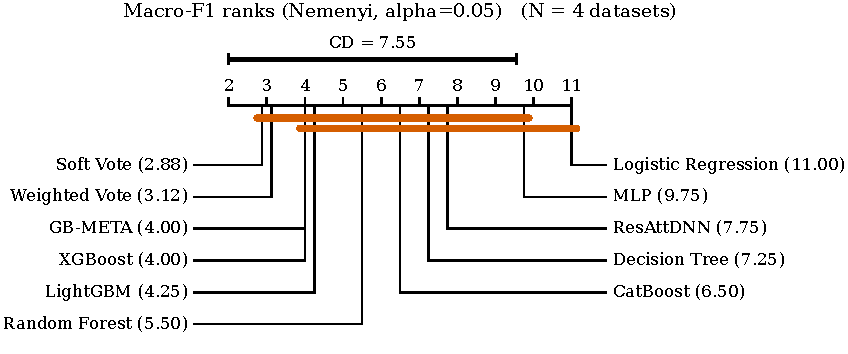
\includegraphics[width=\columnwidth]{fig_critical_difference.pdf}
\caption{Critical-difference diagram over the four benchmarks. Models joined by a
bar are not significantly different at $\alpha{=}0.05$.}
\label{fig:cd}
\end{figure}

\subsection{Ablation}
\begin{table}[t]
\centering
\caption{Ablation of the combination step, measured against the full three-learner stack. A positive $\Delta$ means the simpler configuration is \emph{better}.}
\label{tab:ablation}
\resizebox{\columnwidth}{!}{%
\begin{tabular}{lrrrc}
\toprule
Configuration & Macro-F1 & $\Delta$ vs.\ stack & 95\% CI & Sig. \\
\midrule
\multicolumn{5}{l}{\emph{Edge-IIoTset} (full stack: 0.9243)} \\
\quad Soft vote (no meta-learner) & 0.9166 & $-0.0077$ & $[-0.0113, -0.0041]$ & $\star$ \\
\quad Best single base learner (xgboost) & 0.9164 & $-0.0080$ & $[-0.0114, -0.0042]$ & $\star$ \\
\multicolumn{5}{l}{\emph{NSL-KDD} (full stack: 0.9438)} \\
\quad Soft vote (no meta-learner) & 0.9667 & $+0.0229$ & $[+0.0022, +0.0461]$ & $\star$ \\
\quad Best single base learner (xgboost) & 0.9658 & $+0.0220$ & $[+0.0011, +0.0452]$ & $\star$ \\
\multicolumn{5}{l}{\emph{ToN-IoT} (full stack: 0.9423)} \\
\quad Soft vote (no meta-learner) & 0.9385 & $-0.0038$ & $[-0.0083, +0.0009]$ &  \\
\quad Best single base learner (lightgbm) & 0.9417 & $-0.0006$ & $[-0.0051, +0.0044]$ &  \\
\multicolumn{5}{l}{\emph{UNSW-NB15} (full stack: 0.6027)} \\
\quad Soft vote (no meta-learner) & 0.6322 & $+0.0295$ & $[+0.0163, +0.0439]$ & $\star$ \\
\quad Best single base learner (lightgbm) & 0.6241 & $+0.0214$ & $[+0.0103, +0.0351]$ & $\star$ \\
\bottomrule
\end{tabular}}

\vspace{2pt}
{\footnotesize\raggedright $\star$ = 95\% bootstrap interval excludes zero.\par}
\end{table}

Table~\ref{tab:ablation} removes the learned combination. On Edge-IIoTset the
meta-learner is worth $+0.0077$ macro-F1 over a soft vote. On NSL-KDD and
UNSW-NB15 the soft vote is \emph{better} by $+0.0229$ and $+0.0295$, both with
intervals excluding zero. Two further variants move nothing measurable anywhere:
replacing log-odds meta-features with raw probabilities, and leave-one-out over
the three base learners, which changes Edge-IIoTset macro-F1 by at most 0.0005
with every interval spanning zero. No base learner is individually necessary.

\textbf{Bayesian optimisation.} Fifteen Optuna~\cite{akiba2019optuna} trials on
LightGBM improve validation macro-F1 by $+0.0032$ and \emph{test} macro-F1 by
$+0.0024$, for 212\,s of search, which is within the seed-to-seed spread. Tuning
is not where the headroom is on this benchmark.

\subsection{Seed variance}
Across three seeds the standard deviation of macro-F1 is 0.0026--0.0052 for
GB-\textsc{Meta} and up to 0.0134 for the weaker models. The comparison that
matters is against the differences being claimed: on NSL-KDD the soft vote's
seed-to-seed standard deviation is 0.0100, \emph{larger} than the entire
GB-\textsc{Meta}--XGBoost gap of 0.0072 that the ranking turns on. Applying the
Nadeau--Bengio corrected paired $t$-test against the strongest base learner on
each benchmark finds no significant GB-\textsc{Meta} advantage anywhere
(Edge-IIoTset $p{=}0.124$, NSL-KDD $p{=}0.402$, ToN-IoT $p{=}0.397$), and on
UNSW-NB15 it rejects in the opposite direction ($\Delta{=}{-}0.0214$,
$t{=}{-}13.79$, $p{=}0.005$). Per-model, per-seed values are released with the
artefacts.

\subsection{Confusion, ROC, precision-recall and calibration}

\begin{figure*}[t]
\centering
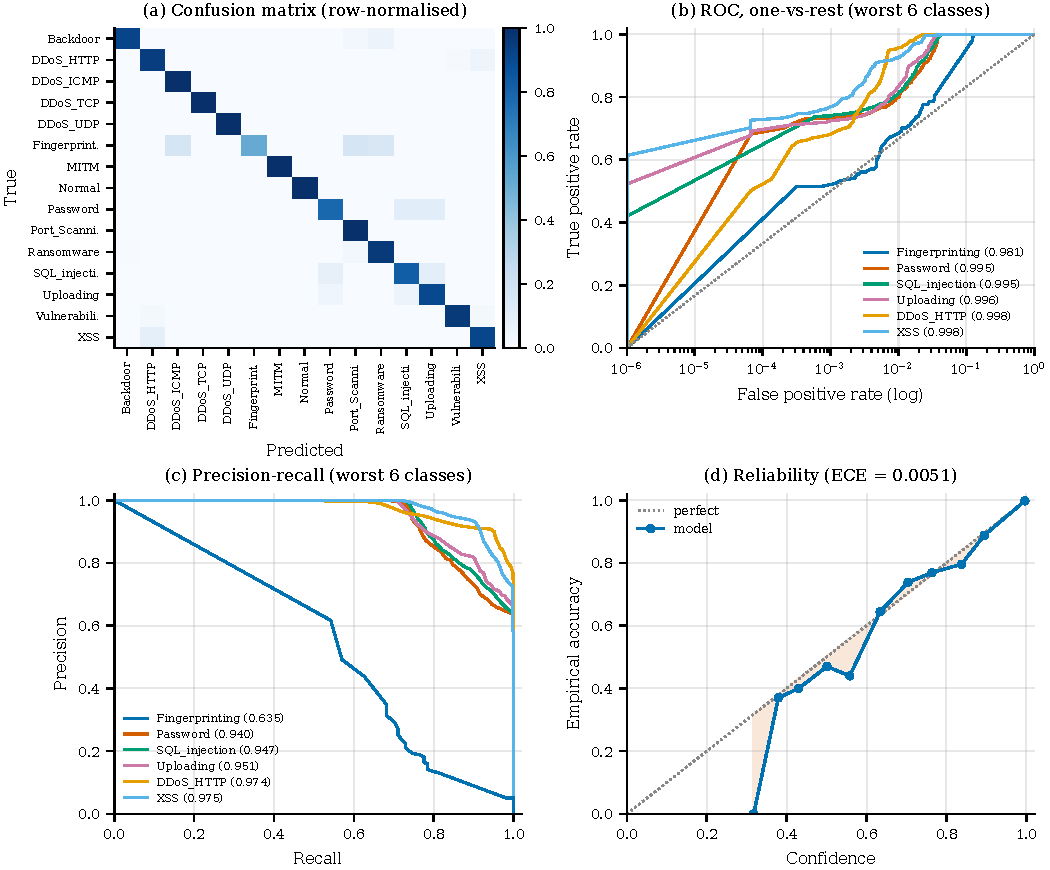
\includegraphics[width=0.70\textwidth]{fig_panel_edge_iiotset_gbmeta.pdf}
\caption{GB-\textsc{Meta} on Edge-IIoTset: (a) row-normalised confusion matrix,
(b) one-vs-rest ROC, (c) precision-recall and (d) reliability. Panels (b) and (c)
show the six weakest classes.}
\label{fig:panel}
\end{figure*}

Figure~\ref{fig:panel} characterises the classifier beyond a single score. The
confusion matrix is row-normalised, since raw counts under a 15.7\% majority
class would say nothing about the minority ones, and shows the errors
concentrated in Fingerprinting, Password and SQL\_injection rather than spread
across the matrix. The ROC axis is logarithmic in the false-positive rate, the only scale on which curves all exceeding 0.98 AUC are distinguishable. Panels (b) and (c) show why AUC alone would mislead: Fingerprinting reaches 0.981 AUC but only 0.635 average precision, since AUC is insensitive to the class prior and precision is not. Panel (d) is the axis on which
GB-\textsc{Meta} is unambiguously best, and the most operationally relevant, since
an alert-triage pipeline consumes confidence scores rather than arg-maxes.

\subsection{Comparison with published results}
\begin{table}[t]
\centering
\caption{Published results on Edge-IIoTset. \emph{Dedup} and \emph{Sig.} record whether duplicates were removed globally and whether any significance test is reported.}
\label{tab:priorart}
\resizebox{\columnwidth}{!}{%
\begin{tabular}{llrrrll}
\toprule
Method & & Cls. & Acc. & Ma-F1 & Dedup & Sig. \\
\midrule
Lightweight stacking & \cite{abdulkareem2024sel} & 15 & 87.37 & -- & no & no \\
OSEN-IoT & \cite{asif2025osen} & 15 & 99.71 & -- & no & no \\
CST-AFNet & \cite{ishtiaq2025cstafnet} & 15 & 99.97 & $>$99.3 & no & no \\
Soft vote (GBDT) & \cite{gaber2025xcl} & 2 & 100.0 & -- & no & no \\
\midrule
GB-\textsc{Meta} (this work) & & 15 & 94.49 & 92.43 & global & yes \\
\bottomrule
\end{tabular}}
\end{table}

Table~\ref{tab:priorart} sets GB-\textsc{Meta} against published Edge-IIoTset
results. Reported accuracies span 87.37\% to 100\% on nominally the same benchmark, a spread no modelling difference accounts for, and none removes duplicates globally or reports a significance test. Our audit prices that
omission: 18.71\% of test rows are exact copies of training rows before
deduplication, so a score measured without it is part lookup and the rows above
ours are not measuring the same quantity. The axis that does carry across is
macro-F1, which is what moves under this benchmark's 44.6:1 imbalance. Only one
of the five reports it and none attaches an interval, whereas GB-\textsc{Meta}
reaches 92.43\% on the deduplicated split with both an interval and a seed-aware
test behind it.

% ---------------------------------------------------------------------------
\section{Deployment Cost}
\label{sec:cost}

\begin{table}[t]
\centering
\caption{Inference cost and model size on Edge-IIoTset. Measurement protocol is given in Section~\ref{sec:cost}.}
\label{tab:cost}
\resizebox{\columnwidth}{!}{%
\begin{tabular}{lrrrrrrr}
\toprule
Model & Macro-F1 & p50 (ms) & p99 (ms) & Peak (s$^{-1}$) & Size (MB) & Trees & Train (s) \\
\midrule
Decision Tree & 0.9189 & 0.148 & 0.271 & 4,234,029 & 0.011 & 1 & 0.3 \\
MLP & 0.9117 & 0.314 & 0.358 & 665,637 & 0.192 & 50,703 & 42.7 \\
XGBoost & 0.9164 & 0.358 & 0.575 & 237,566 & 0.909 & 2,325 & 13.1 \\
CatBoost & 0.9150 & 0.460 & 0.517 & 476,633 & 1.891 & 380 & 55.7 \\
LightGBM & 0.9155 & 1.178 & 1.579 & 199,859 & 1.038 & 630 & 3.4 \\
GB-META & 0.9243 & 3.100 & 3.621 & 71,517 & 3.846 & -- & 213.3 \\
Random Forest & 0.9180 & 45.252 & 59.435 & 26,290 & 17.600 & 200 & 2.6 \\
\bottomrule
\end{tabular}}

\end{table}


Table~\ref{tab:cost} reports batch-1 p50 and p99 latency over 60 timed
repetitions after 20 warm-up calls, peak throughput from a batch sweep, and
gzip-compressed size. The stack is profiled end to end, including every base model's forward pass. On Edge-IIoTset
GB-\textsc{Meta} reaches 0.9243 macro-F1 at 3.10\,ms and 3.85\,MB against a
single depth-12 decision tree at 0.9189, 0.15\,ms and 0.011\,MB: the stack buys
0.0054 macro-F1 for 20.9$\times$ the latency and 350$\times$ the size. Training
cost tells the same story: 213.3\,s, of which 141.2\,s is the out-of-fold
generation the meta-learner requires, against 0.3\,s.

Three quantities are deliberately absent. CPU energy would be a TDP estimate
presented as a measurement, since RAPL/\texttt{powercap} counters are unreadable
in the measurement environment. Embedded latency is not extrapolated, no
calibrated Cortex-A72-versus-x86 ratio existing for tree ensembles. And no int8
speed-up is reported, because ONNX Runtime's quantisation registry has no entry
for \texttt{TreeEnsemble} operators.

% ---------------------------------------------------------------------------
\section{Robustness and Concept Drift}
\label{sec:robust}

\textbf{Input perturbation.} We measure macro-F1 on Edge-IIoTset under increasing
Gaussian noise applied to the scaled features, and under per-row zeroing of a
fraction of them. The first is a proxy for an adversary able to manipulate
observable flow statistics, the second for sensor dropout and partial telemetry
loss. This produces the sharpest separation anywhere in the study, and it does
not favour the stack. At $\sigma{=}0.1$, one tenth of an inter-quartile
range, XGBoost and LightGBM collapse from 0.92 to 0.28 and 0.31 macro-F1, while
CatBoost retains 0.82 and a plain decision tree 0.76. GB-\textsc{Meta} inherits an
intermediate 0.60: the meta-learner spreads weight across three base models, two
of them brittle, so averaging buys some protection but far less than selecting
the robust one would. Under 20\% feature masking the ordering is the same
(CatBoost 0.73, GB-\textsc{Meta} 0.66, decision tree 0.52). If robustness to
perturbed input is an operational requirement, CatBoost alone dominates the
ensemble built on top of it. Full sweeps are released with the artefacts.

The immutability mask matches only 1 of 58 Edge-IIoTset features, whose protocol-level columns do not follow flow-statistics naming conventions, so the sweep is a worst case rather than a realisable attack.

\textbf{Concept drift.} ToN-IoT is the only benchmark here with a usable
timestamp, since Edge-IIoTset's \texttt{frame.time} was corrupted at publication
by an unquoted comma and NSL-KDD carries none, so it is the only candidate for a
chronological evaluation. Running the standard protocol on it characterises the benchmark rather than the models. Its capture is organised by attack campaign rather than interleaved, which makes a chronological split
\emph{class-disjoint}: the first 68\% of the capture holds \{normal, ddos, dos,
injection, password, scanning\} and the test period holds \{normal, backdoor,
mitm, ransomware, xss\}. Only the benign class is common, four of five test
classes never appear in training, and 53.7\% of test rows belong to an unseen
class. Every model scores below 0.07 macro-F1, which measures an unreachable
label space rather than degradation over time. Feature statistics confirm it: mean PSI over the 96 encoded features is 0.040 with only 5 above the
conventional 0.25 threshold, so the covariate distribution barely moves while the
prior changes almost completely. A chronological split of ToN-IoT is therefore an
open-set recognition task, and an AUT computed on it scores that rather than
drift. We report this as a property of the benchmark: temporal evaluations on
ToN-IoT should state their class overlap.

% ---------------------------------------------------------------------------
\section{Discussion and Threats to Validity}

\textbf{Scale.} Each benchmark is subsampled to 80{,}000 rows. Rerunning
Edge-IIoTset at full scale over the same three seeds (152{,}196 rows after
deduplication) improves every model, most by 0.002 to 0.007 macro-F1, and
preserves the ordering: GB-\textsc{Meta} remains first of eleven at
$0.9238 \pm 0.0046$. The subsample sets the absolute scores, not the comparison.
\textbf{Power.} Four benchmarks is few: Friedman rejects, but Nemenyi separates 2
of 55 pairs and Wilcoxon cannot reject at this $N$.
\textbf{Tuning.} Base learners use fixed, documented hyper-parameters rather than
per-dataset tuning, and any tuning procedure must be applied to the baselines too.
\textbf{Class merging.} Classes below 30 rows are folded into one rare category.
This touches one benchmark: 10 of NSL-KDD's 23 classes, together 92 rows or 0.073\% of it. Edge-IIoTset, ToN-IoT and UNSW-NB15 are untouched, their smallest classes holding 358, 646 and 127 rows, so macro-F1 stays comparable across the four.
\textbf{Host.} Timing is CPU-only on a two-core host and should be read as
relative.

% ---------------------------------------------------------------------------
\section{Conclusion}

GB-\textsc{Meta} is the best-performing of eleven models on Edge-IIoTset under a
leakage-audited protocol, on macro-F1 and on calibration, with the margin
concentrated in the minority classes that make this benchmark hard. The ablation
attributes that result to the learned combination step rather than to the choice
of base learners, which is the design claim the paper set out to test.

The advantage is benchmark-specific, and the evaluation says where it applies: we
recommend GB-\textsc{Meta} for calibrated minority-class detection on IoT traffic
of this kind, and CatBoost alone where robustness to perturbed input is an
operational requirement. Establishing a claim at this resolution needs the
protocol as much as the model, since the seed-to-seed spread of these models
overlaps the differences routinely used to rank them. We release both.

\section*{Reproducibility}

Code, cached probability matrices, tables and figures are available at
\url{https://github.com/ANONYMISED}. Every table, test and figure is recomputed
from the cached matrices by one script; the complete study runs in 52 minutes on
the reference host.

% ---------------------------------------------------------------------------
% Bibliography set one size down -- standard practice in IEEE conference
% submissions and the difference between six and seven pages here.
{\footnotesize
\bibliographystyle{IEEEtran}
\bibliography{references}
}

\end{document}
